\documentclass[paper=letter, fontsize=12pt]{article}

\usepackage{amsmath,amsfonts,amsthm, amssymb} % Math packages
\usepackage{stmaryrd}
\usepackage[shortlabels]{enumitem}
\usepackage[pdftex]{graphicx}
\usepackage{booktabs}
\usepackage{placeins}
\usepackage{algpseudocode}
\usepackage[margin=1in]{geometry}
\usepackage{listings}
\usepackage{mdframed}
\usepackage{tcolorbox}
\usepackage{float}
\usepackage{subcaption}
\usepackage{url}
\usepackage{hyperref}

\usepackage{mathtools}
\DeclarePairedDelimiterX{\norm}[1]{\lVert}{\rVert}{#1}
\DeclarePairedDelimiterX{\abs}[1]{\lvert}{\rvert}{#1}
\DeclareMathOperator*{\argmin}{arg\,min}
\DeclareMathOperator{\spn}{span}
\DeclareMathOperator{\rct}{rect}
\DeclareMathOperator{\support}{support}
\DeclareSymbolFont{matha}{OML}{txmi}{m}{it}% txfonts
\DeclareMathSymbol{\varv}{\mathord}{matha}{118}
\DeclareMathOperator{\E}{\mathbb{E}}
\DeclareMathOperator{\Tr}{Tr}

\newcommand{\ceil}[1]{\lceil #1 \rceil}
\newcommand{\floor}[1]{\lfloor #1 \rfloor}
\newcommand{\Lapl}{\mathcal{L}}
\newcommand{\reals}{\mathbb{R}}
\newcommand{\complexes}{\mathbb{C}}
\newcommand{\ints}{\mathbb{Z}}
\newcommand{\innerp}[2]{\langle #1, #2 \rangle}
\newcommand{\vecii}[2]{\begin{bmatrix} #1 \\ #2 \end{bmatrix}}
\newcommand{\veciii}[3]{\begin{bmatrix} #1 \\ #2 \\ #3 \end{bmatrix}}
\newcommand{\rect}[1]{\rct \left( #1 \right)}
\newcommand{\pw}[1]{\begin{cases} #1 \end{cases}}
\newcommand{\Mod}[1]{\ \text{mod}\ #1}
\newcommand{\sumN}{\sum\limits_{n=0}^{N-1}}
\newcommand{\sumK}{\sum\limits_{k=0}^{N-1}}
\newcommand\given[1][]{\:#1\vert\:}

\graphicspath{{img/}}

\title{CS 543 - Progress Report}
\author{
        Dario Aranguiz \\
        Cu-Khoi-Nguyen Mac
        }
\date{\today}


%%% Begin document
\begin{document}
\maketitle
% \pagebreak

\section{Updated statement of the project definition and goals}

\section{Current member roles and collaboration strategies}

\section{Proposed approach}

\section{Data}
Following the proposed approach by Eitel et al. \cite{Eitel2015}, we decide to use Washington's RGB-D object dataset \cite{Lai2011} for training and testing. The dataset contains 300 household objects (instances) divided into 51 categories. Each instance has three different takes, each records a full turn-around rotation of the object. A sample of the full database includes images of color, depth, mask (as seen in Figure \ref{fig:banana}), and a text file recording the top-left corner of the object.

\begin{figure}[htbp]
	\centering
	\begin{subfigure}[b]{0.32\linewidth}
		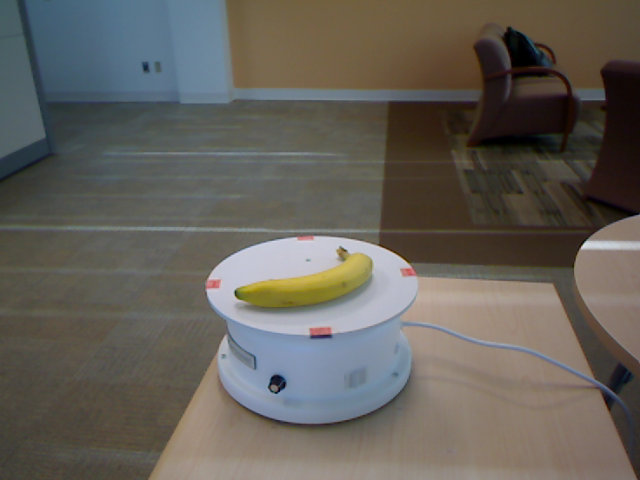
\includegraphics[width=\textwidth]{banana_1_1_1}
		\caption{Color image}
	\end{subfigure}
	\begin{subfigure}[b]{0.32\linewidth}
		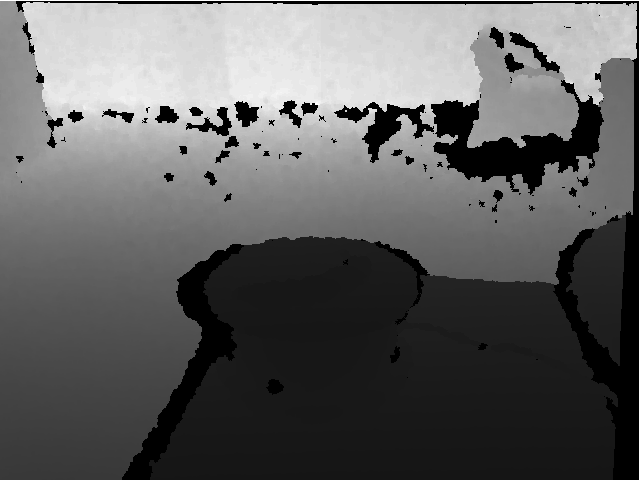
\includegraphics[width=\textwidth]{banana_1_1_1_depth}
		\caption{Depth image}
	\end{subfigure}
	\begin{subfigure}[b]{0.32\linewidth}
		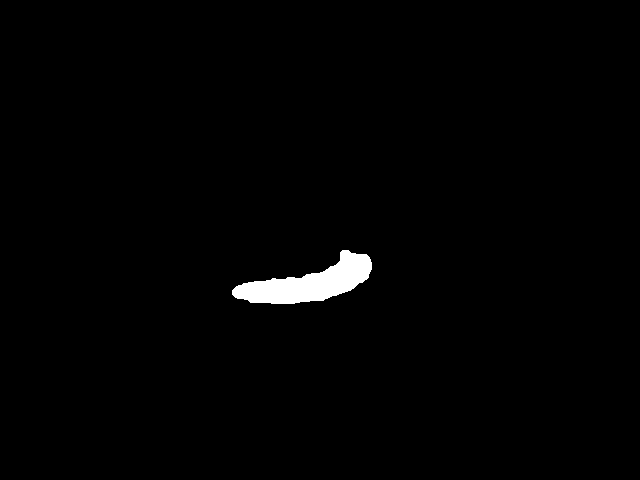
\includegraphics[width=\textwidth]{banana_1_1_1_mask}
		\caption{Mask}
	\end{subfigure}
	
	\caption{A banana sample of Washington's RGB-D object dataset. The depth image is rescaled to the range [0, 255] to visual the information.}
	\label{fig:banana}
\end{figure}

To speed up the process of testing our system's runnability, we pick out 15 instances from 5 different categories (3 each), namely \texttt{apple}, \texttt{ball}, \texttt{banana}, \texttt{bell\_pepper}, and \texttt{binder}. After the system is fully functional, we will expand the training list to the whole dataset.


\section{Initial results}
\subsection{Data preprocessing}
We use the provided masks and top-left corners to remove unnecessary information from color and depth images (Figure \ref{fig:banana_crop}). Top bottom-right corner if dynamically found, depending on each sample. According to Eitel et al. \cite{Eitel2015}, they convert the depth images into color ones using colorjet mapping as they want to have the same training mechanism for both color and depth. We inherit this idea and apply the same depth colorizing technique. The images are then rescaled to 227x227 (Figure \ref{fig:banana_resize}) by replicating the longer side from the cropped images. This help to maintain the object in the center without deformation after rescaling.

\begin{figure}[htbp]
	\centering
	\begin{subfigure}[b]{0.32\linewidth}
		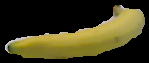
\includegraphics[width=\textwidth]{banana_1_1_1_crop}
		\caption{Color image}
	\end{subfigure}
	\begin{subfigure}[b]{0.32\linewidth}
		
\includegraphics[width=\textwidth]{banana_1_1_1_depth_crop}
		\caption{Depth image}
	\end{subfigure}
	\caption{Cropping banana sample after applying mask.}
	\label{fig:banana_crop}
\end{figure}

\begin{figure}[htbp]
	\centering
	\begin{subfigure}[b]{0.32\linewidth}
		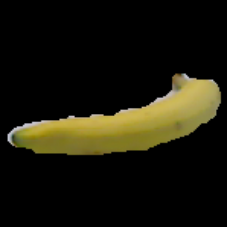
\includegraphics[width=\textwidth]{banana_1_1_1_resize}
		\caption{Color image}
	\end{subfigure}
	\begin{subfigure}[b]{0.32\linewidth}
		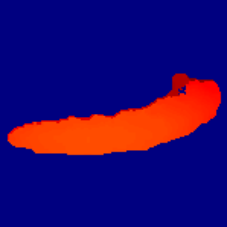
\includegraphics[width=\textwidth]{banana_1_1_1_depth_resize}
		\caption{Depth image (after colorizing)}
	\end{subfigure}
	\caption{Rescaling banana sample to 227x227 by replicating the longer side.}
	\label{fig:banana_resize}
\end{figure}

\subsection{Model architecture}
Figure \ref{fig:architecture_eitel} illustrates the network architecture proposed by Eitel et al. \cite{Eitel2015}. There are two separate stream models, corresponding to color and depth channels. Each stream contains 5 convolution (from \texttt{conv-1} to \texttt{conv-5}) and 2 fully connected layers (\texttt{fc6} and \texttt{fc7}). The streams are fused together by one fusion layer (\texttt{fc-fus}) and classified by \texttt{class} layer.
\begin{figure}[htbp]
	\centering
	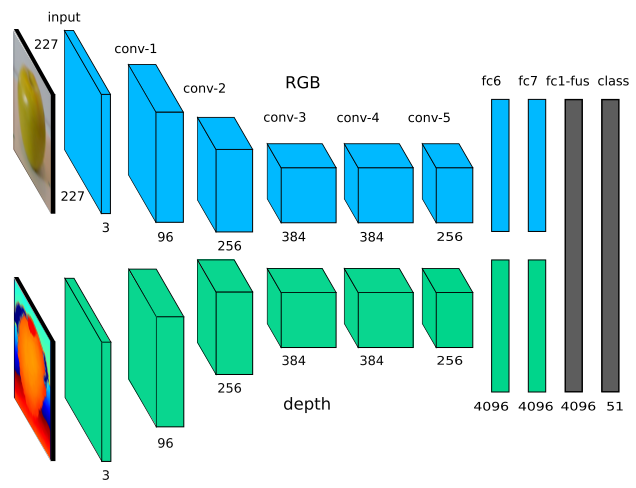
\includegraphics[width=.7\textwidth]{architecture}
	\caption{Model architecture proposed by Eitel et al. \cite{Eitel2015}.}
	\label{fig:architecture_eitel}
\end{figure}

Figure \ref{fig:fusion_model} shows our model, constructed by following the description in Figure \ref{fig:architecture_eitel}. The model is plotted using visualizer package of Keras. Using Keras, each stream is constructed using \texttt{Sequential()} model and the fusion layer is created by \texttt{Merge()} layer. We propose to augment each convolutional layer (\texttt{Convolution2D()}) with a maxpooling (\texttt{MaxPolling2D()}) and a dense sampling layer (\texttt{Dense()}) to reduce the risk of over-fitting and decrease memory usage.

In fact, there are two different training process: one to find the weights of stream model and one for the fusion model. To train a stream model, we create an architecture similar to a branch in Figure \ref{fig:fusion_model} and add one classifier at the end (Figure \ref{fig:stream_model}). The weights of trained streams are reused to initialize the two branches of the whole network.

\begin{figure}[htbp]
\centering
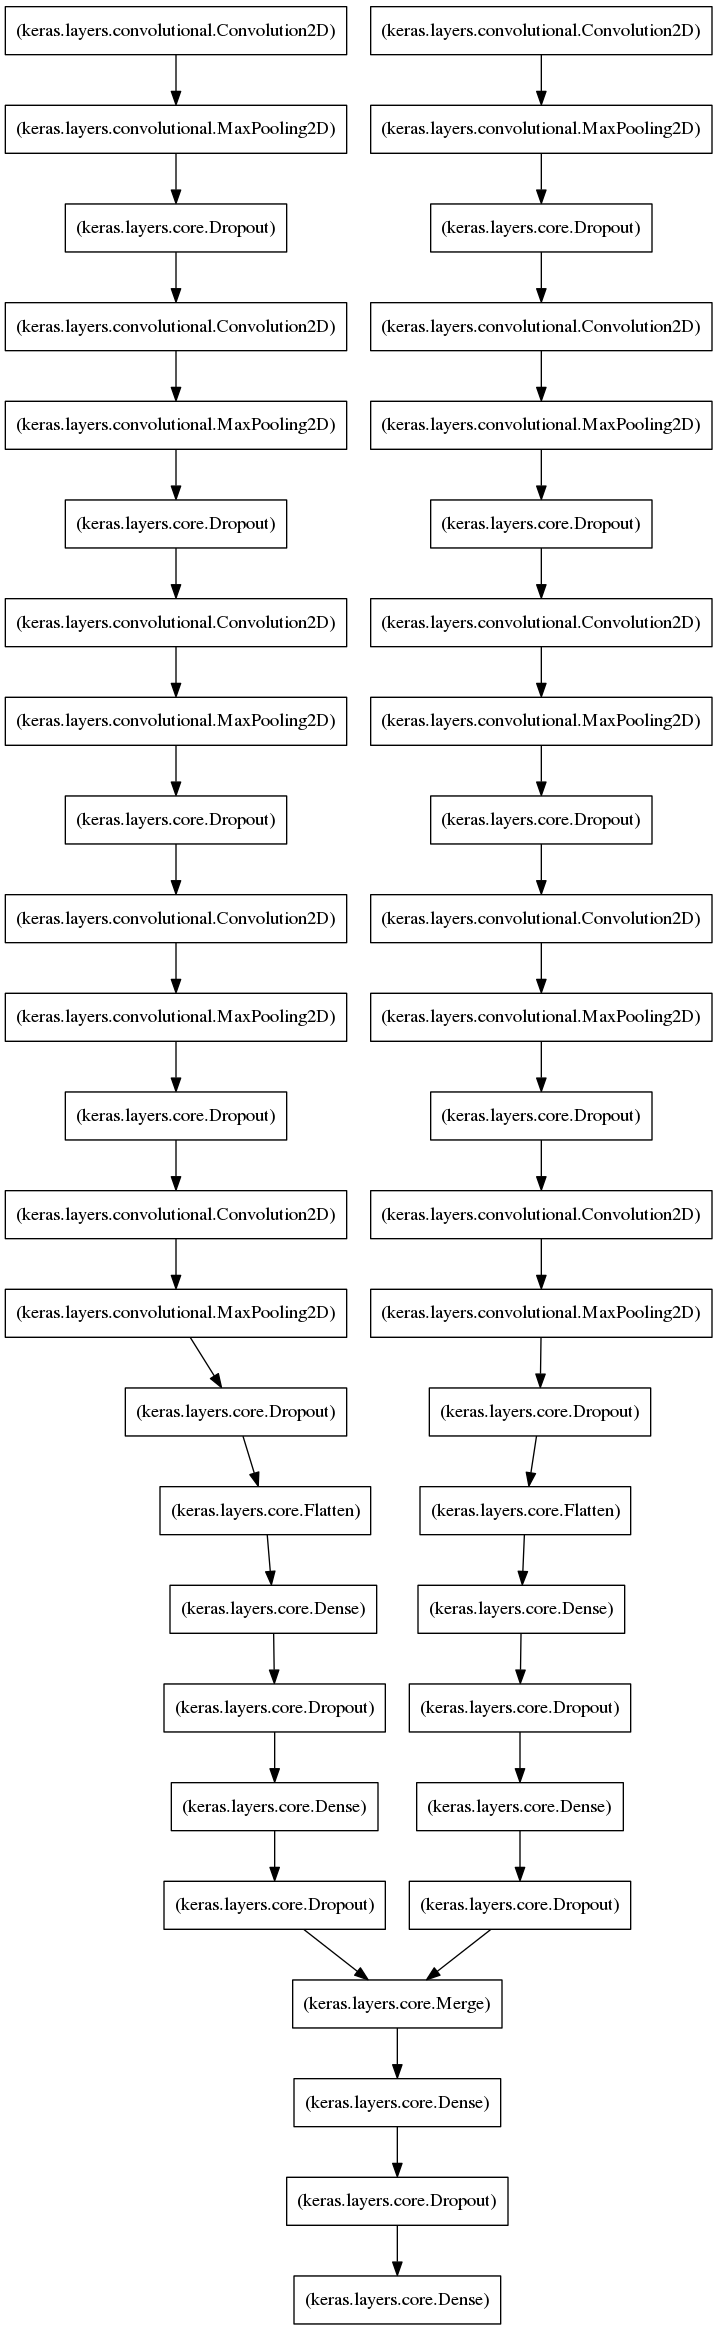
\includegraphics[width=.42\textwidth]{fusion_model}
\caption{Fusion model with RGB and depth streams.}
\label{fig:fusion_model}
\end{figure}

\begin{figure}[htbp]
	\centering
	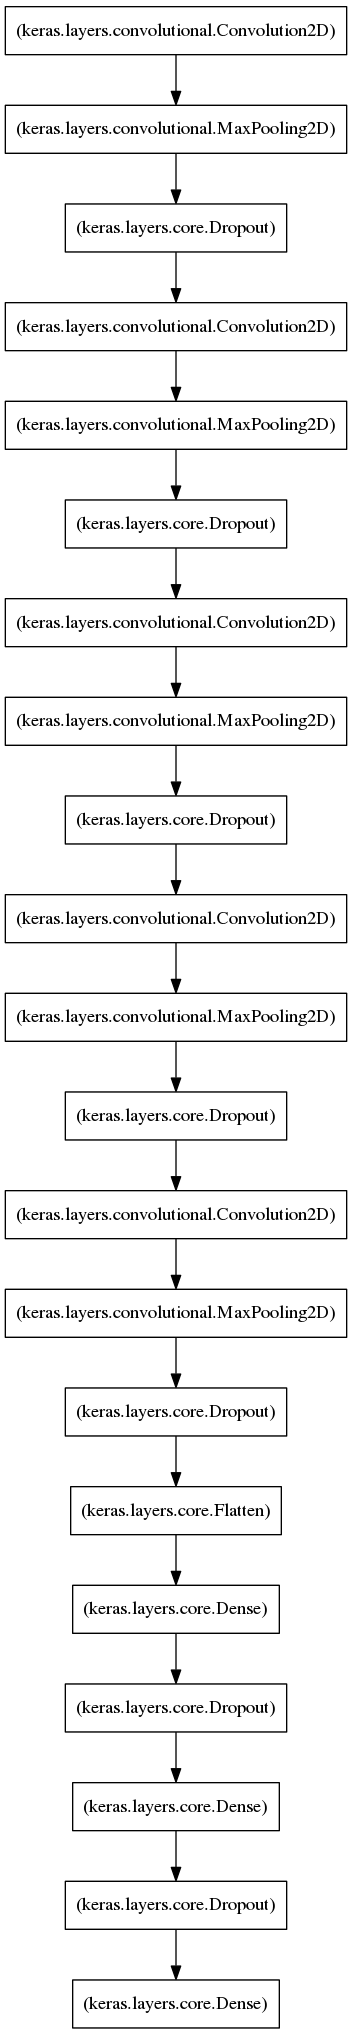
\includegraphics[width=.24\textwidth]{stream_model}
	\caption{Single stream model.}
	\label{fig:stream_model}
\end{figure}

\subsection{Other accomplishments}
Beside data preprocessing and model construction, we have also successfully configured a GPU environment for Keras/Theano to speed up training process. In addition, the paper mentions about using CaffeNet to initialize the network. However, this pretrained network has to be converted to Keras format before loading. We utilize a modified version of Keras that includes conversion package, provided by Bolanos \cite{Bolanos2016}.

\section{Current reservations and questions}
(if any)

\bibliographystyle{ieeetr}
\bibliography{mybib}


%%% End document
\end{document}